% Generated by make_fig_b_results.py from committed results. Do not edit by hand.
\documentclass[border=2pt]{standalone}
\usepackage[T1]{fontenc}\usepackage{newtxtext,newtxmath}\usepackage[varqu,scaled=0.95]{zi4}
\usepackage{pgfplots}\pgfplotsset{compat=1.18}\usepgfplotslibrary{groupplots}
\definecolor{cblue}{HTML}{0072B2}\definecolor{cver}{HTML}{D55E00}\definecolor{cora}{HTML}{E69F00}
\definecolor{cgreen}{HTML}{009E73}\definecolor{cgrey}{HTML}{999999}
\pgfplotsset{every axis/.append style={font=\footnotesize, tick label style={font=\scriptsize},
  label style={font=\footnotesize}, legend style={font=\scriptsize, draw=none, fill=none},
  axis lines*=left, grid style={black!8}}}
\begin{document}

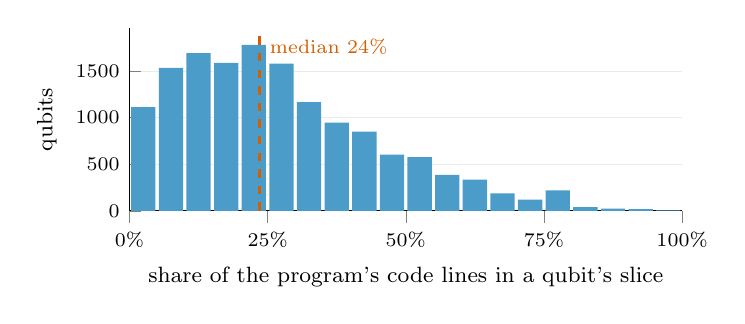
\begin{tikzpicture}
\begin{axis}[width=8.6cm, height=3.9cm, ybar, bar width=4.4, xmin=0, xmax=100, ymin=0, enlarge x limits=false, xtick={0,25,50,75,100}, xticklabel={\pgfmathprintnumber{\tick}\%}, ymajorgrids, xlabel={share of the program's code lines in a qubit's slice}, ylabel={qubits}, scaled y ticks=false, yticklabel style={/pgf/number format/1000 sep={}}]
\addplot[fill=cblue!70, draw=none] coordinates {(2.5,1115) (7.5,1537) (12.5,1694) (17.5,1589) (22.5,1784) (27.5,1581) (32.5,1169) (37.5,947) (42.5,852) (47.5,603) (52.5,578) (57.5,386) (62.5,334) (67.5,186) (72.5,121) (77.5,219) (82.5,40) (87.5,22) (92.5,19) (97.5,5)};
\draw[cver, line width=0.9pt, dashed] ({axis cs:23.53,0}|-{rel axis cs:0,0}) -- ({axis cs:23.53,0}|-{rel axis cs:0,1}) node[anchor=north west, font=\scriptsize, text=cver] {median 24\%};
\end{axis}
\end{tikzpicture}
\end{document}
